\documentclass[11pt]{article}
\usepackage[T1]{fontenc}
\usepackage[utf8]{inputenc}
\usepackage{lmodern,microtype}
\usepackage[margin=1in]{geometry}
\usepackage{amsmath,amssymb,amsthm,mathtools}
\usepackage{booktabs,array,longtable}
\usepackage[dvipsnames]{xcolor}
\usepackage{tikz}
\usepackage{enumitem,needspace}
\usepackage{fancyhdr}
\usepackage{listings}
\usepackage[colorlinks=true,linkcolor=MidnightBlue,citecolor=MidnightBlue,urlcolor=MidnightBlue]{hyperref}
\usepackage[nameinlink,noabbrev]{cleveref}
\hypersetup{pdftitle={Largest Simplex Faces under Ordinal Sums},pdfauthor={Research draft prepared for Vladimir Reshetnikov},pdfsubject={Exact formulae and a sharp extremal theorem for series-parallel posets}}
\newtheorem{theorem}{Theorem}[section]
\newtheorem{lemma}[theorem]{Lemma}
\newtheorem{proposition}[theorem]{Proposition}
\newtheorem{corollary}[theorem]{Corollary}
\theoremstyle{definition}
\newtheorem{definition}[theorem]{Definition}
\newtheorem{example}[theorem]{Example}
\newtheorem{remark}[theorem]{Remark}
\newcommand{\OO}{\mathcal O}
\newcommand{\CC}{\mathcal C}
\newcommand{\sO}{s_{\OO}}
\newcommand{\sC}{s_{\CC}}
\newcommand{\RR}{\mathbb R}
\newcommand{\SP}{\mathsf{SP}}
\newcommand{\conv}{\operatorname{conv}}
\newcommand{\rk}{\operatorname{rank}}
\newcommand{\minusinf}{-\infty}
\newcommand{\one}{\mathbf 1}
\newcommand{\zero}{\mathbf 0}
\newcommand{\A}[1]{\mathsf A_{#1}}
\newcommand{\pospart}[1]{\left(#1\right)_{+}}
\newcommand{\smat}[4]{\left(\begin{smallmatrix}#1&#2\\#3&#4\end{smallmatrix}\right)}
\DeclareMathOperator*{\maxp}{max}
\setlength{\emergencystretch}{2em}
\setlength{\headheight}{14pt}
\pagestyle{fancy}
\fancyhf{}
\fancyhead[L]{\small Largest simplex faces under ordinal sums}
\fancyhead[R]{\small Research draft}
\fancyfoot[C]{\thepage}
\setcounter{tocdepth}{2}
\lstset{basicstyle=\ttfamily\small,columns=fullflexible,keepspaces=true,breaklines=true,frame=single,rulecolor=\color{black!25},showstringspaces=false}
\title{\textbf{Largest Simplex Faces under Ordinal Sums}\\[0.45em]
\large Exact formulae for series--parallel posets,\\a path-matching interpretation, and a sharp extremal gap}
\author{Research draft prepared for Vladimir Reshetnikov}
\date{20 September 2026}

\begin{document}
\maketitle
\begin{abstract}
For a finite poset $P$, let $\sO(P)$ and $\sC(P)$ denote the largest dimensions of simplex faces of its order and chain polytopes. A recent paper of Freij-Hollanti and Lundstr\"om explicitly asks for formulae for these quantities, including for series--parallel posets. We give an exact constant-state recursion on a series--parallel decomposition: two numbers suffice for the chain polytope, and four endpoint-refined numbers suffice for the order polytope. The latter reduce, after normalization, to eight states. For an ordinal sum of antichains of sizes $a_1,\ldots,a_r$, the formula becomes nonrecursive: $\sO=r+\nu$, where $\nu$ is the cardinality of a maximum capacitated matching on the path of layers, and $\sC=r+\max(0,k-1)$, where $k$ counts the nonsingleton layers. We also establish the sharp bound
\[
\max_{\substack{P\in\SP\\|P|=n}}
\bigl(\sC(P)-\sO(P)\bigr)
=\left\lfloor\frac{n-2}{3}\right\rfloor\qquad(n\ge2).
\]
The arguments use elementary face geometry and a completely displayed finite transition table. Exact computations from defining inequalities verify the endpoint states on every series--parallel isomorphism type through six elements, represented by 1,977 naturally labelled instances. Reproducible code and certificates accompany the article. The results are presented as a proposed solution of the series--parallel case, not as a peer-reviewed priority claim or a solution for arbitrary finite posets.
\end{abstract}

\section*{Status and scope}
The proofs below are mathematical arguments, not inferences from numerical fitting. Their novelty has not been independently established, and the draft has not been peer reviewed or formally verified. The principal bibliographic check is unusually concrete: the version of record of the source paper, published on 2 September 2026, retains the open question in its concluding paragraph. For general series--parallel posets our answer is an explicit recursion; for ordinal sums of antichains it is an explicit nonrecursive formula. No theorem about infinite ordinals or large cardinals is claimed.

\clearpage
\tableofcontents
\clearpage

\section{The question and the main results}\label{sec:intro}

Order theory connects to polyhedral geometry through two constructions introduced by Stanley~\cite{Stanley1986}. Both encode a finite partially ordered set as a convex polytope, but their face structures can differ. Here the invariant of interest is the largest dimension of a face that is a simplex. This is a restriction on the \emph{face lattice}: it is not the largest dimension of a simplex that can merely be placed inside the polytope.

\subsection{A documented open problem}
Freij-Hollanti and Lundstr\"om~\cite{FHL2026}, in the last mathematical paragraph of Section~4, ask for a formula for the largest simplex-face dimension of the order and chain polytopes. They explicitly identify series--parallel posets as a class for which this appears open. The same paper proves a stronger, dimension-by-dimension inequality between numbers of simplex faces for a recursively defined class containing the series--parallel posets. In particular, its results already imply $\sO(P)\le\sC(P)$ in our class. We do not claim that inequality as new.

The literature search was checked against the published article, its arXiv version~\cite{FHLpreprint}, and the related simplex-face and polytope-decomposition papers~\cite{FHL2024,Mori2025,MoriOhsugi2026}. No later resolution of the stated formula question was located. This is evidence for the choice of problem, not an exhaustive certification of priority.

The useful structural feature is the availability of two recursive operations: disjoint union and ordinal sum. Under disjoint union the relevant polytopes become products; under ordinal sum they become two polytopes joined at a distinguished vertex. The remaining difficulty is to remember enough information about that vertex when another ordinal sum is taken.

\subsection{Results at a glance}
Let $\A a$ be an antichain with $a$ elements, and let $\SP$ be the nonempty finite posets constructed from a singleton by disjoint union and ordinal sum.

\begin{theorem}[Exact evaluation]\label{thm:overview-recursion}
Given a binary series--parallel decomposition of an $n$-element poset $P$, both $\sO(P)$ and $\sC(P)$ can be computed with $O(n)$ integer additions and comparisons. The order-polytope calculation maintains four endpoint-refined values, which normalize to the eight states in \cref{tab:states}. The chain-polytope calculation maintains the height and one origin-avoiding value.
\end{theorem}

\begin{theorem}[Ordinal sums of antichains]\label{thm:overview-layers}
Suppose
\[
P=\A{a_1}<\A{a_2}<\cdots<\A{a_r},\qquad a_i\ge1.
\]
Let $k=\#\{i:a_i\ge2\}$. On the path with vertices $1,\ldots,r$, give vertex $i$ capacity $b_i=\min(a_i-1,2)$, and let $\nu$ be the maximum cardinality of an edge set whose selected degree at each vertex is at most its capacity. Then
\[
\boxed{\sO(P)=r+\nu,\qquad \sC(P)=r+\max(0,k-1).}
\]
Moreover, $\nu$ is an explicit sum of ceilings of half-path lengths; see \cref{cor:conflict}.
\end{theorem}

\begin{theorem}[Sharp extremal gap]\label{thm:overview-gap}
For every $P\in\SP$ with $n\ge2$ elements,
\[
0\le\sC(P)-\sO(P)\le\left\lfloor\frac{n-2}{3}\right\rfloor.
\]
For every $n\ge2$ there is such a poset attaining equality in the upper bound. For $n=1$, both dimensions are $1$ and the gap is $0$.
\end{theorem}

The point of the second and third results is to go beyond a generic algorithm that enumerates vertices or faces. They identify a small combinatorial optimization problem for the layered case and determine the exact worst discrepancy over the entire series--parallel class.

\section{Definitions and elementary facts}\label{sec:definitions}

All posets in this article are finite and nonempty unless stated otherwise. If $A$ and $B$ have disjoint ground sets, their \emph{disjoint union} $A\sqcup B$ adds no comparisons between the factors. Their \emph{ordinal sum} $A<B$ keeps all internal comparisons and declares every element of $A$ smaller than every element of $B$. Parentheses in iterated ordinal sums may be suppressed. The height $h(P)$ is the maximum \emph{number of elements} in a chain, rather than its number of strict inequalities.

Our use of ``series--parallel'' refers to these recursive operations on posets, not to an unrelated convention about two-terminal electrical networks. The classical graph-theoretic background is discussed by Jung~\cite{Jung1978}; the constructive definition alone suffices for every proof here.

\begin{definition}
For a poset $P$, its order polytope and chain polytope are
\begin{align}
\OO(P)&=\{x\in[0,1]^P:x_p\le x_q\text{ whenever }p\le_P q\},\label{eq:orderdef}\\
\CC(P)&=\{x\in\RR_{\ge0}^P:\textstyle\sum_{p\in K}x_p\le1
                    \text{ for every chain }K\subseteq P\}.\label{eq:chaindef}
\end{align}
For a polytope $Q$, write $s(Q)$ for the maximum dimension of a simplex face. We set $\sO(P)=s(\OO(P))$ and $\sC(P)=s(\CC(P))$.
\end{definition}

A face is the set of maximizers of a linear functional; the whole polytope and the empty face are included. A nonempty $d$-simplex has exactly $d+1$ affinely independent vertices. The empty face is treated as a simplex of dimension $-1$. An impossible endpoint requirement receives value $-\infty$, not $-1$. This distinction is essential: an existing empty face is different from a nonexistent face containing a required vertex.

A filter is an upward-closed subset. An antichain is a subset whose distinct elements are pairwise incomparable. We use $\chi_S$ for the characteristic vector of $S$.

\begin{lemma}[Vertices]\label[lemma]{lem:vertices}
The vertices of $\OO(P)$ are the vectors $\chi_F$ for filters $F$. The vertices of $\CC(P)$ are the vectors $\chi_A$ for antichains $A$.
\end{lemma}
\begin{proof}
For the order polytope, the level set $F_t=\{p:x_p\ge t\}$ is a filter for every $t\in(0,1]$, and
\[
x=\int_0^1\chi_{F_t}\,dt.
\]
There are only finitely many distinct level sets, so this is a convex combination of filter vectors. Conversely, each such vector satisfies \eqref{eq:orderdef}.

For the chain polytope, let $x$ satisfy \eqref{eq:chaindef}. Define $t_p$ to be the maximum weight $\sum_{q\in K}x_q$ of a chain strictly below $p$, allowing the empty chain. Associate to $p$ the interval $(t_p,t_p+x_p]$. These intervals lie in $[0,1]$. If $p<q$, then $t_q\ge t_p+x_p$, so their intervals are disjoint. Therefore, for each $t$, the elements whose intervals contain $t$ form an antichain $A_t$. Again,
\[
x=\int_0^1\chi_{A_t}\,dt
\]
is a finite convex combination. Every antichain vector is feasible.

Finally, a $0/1$ vector in a convex set contained in the unit cube cannot be a nontrivial convex combination of other points of that set: each coordinate equal to $0$ or $1$ forces the same coordinate in every point of the combination. Thus all the displayed vectors are vertices, and there are no others.
\end{proof}

This is the familiar vertex description from Stanley's theory~\cite{Stanley1986}; the proof is included to make the later reductions self-contained. In particular, $\zero_P$ and $\one_P$ are distinct vertices of $\OO(P)$, and $\zero_P$ is a distinguished vertex of $\CC(P)$.

\begin{example}[Why the word ``face'' matters]
For an $n$-element antichain, both polytopes are the cube $[0,1]^n$. If $n\ge2$, this cube contains full-dimensional simplices, but its largest simplex faces are only edges. Thus $\sO(\A n)=\sC(\A n)=1$. For an $n$-element chain both polytopes themselves are $n$-simplices, so both invariants equal $n$.
\end{example}

\section{Faces under products and vertex sums}\label{sec:geometry}

We first record the geometric machinery. The vertex-sum construction and its application to ordinal sums are used in~\cite{FHL2024}; the arguments below retain explicit endpoint information.

\begin{lemma}[Products]\label[lemma]{lem:product}
Every nonempty face of $Q\times R$ is $F\times G$ for nonempty faces $F$ and $G$. Such a face is a simplex if and only if one factor is a point and the other is a simplex. Consequently,
\[
s(Q\times R)=\max\{s(Q),s(R)\}.
\]
\end{lemma}
\begin{proof}
A linear functional on the product splits as $\ell(x)+m(y)$, and its maximizing set is the product of the two maximizing sets. If $F$ and $G$ both have positive dimension, each has an edge, and the product of those edges is a quadrilateral face of $F\times G$. A simplex has no quadrilateral face. If one factor is a point, the product is affinely equivalent to the other factor.
\end{proof}

\begin{definition}
Suppose $0$ is a vertex of $Q\subseteq\RR^a$ and $R\subseteq\RR^b$. Their \emph{vertex sum} is
\[
Q\vee R=\conv\bigl((Q\times\{0\})\cup(\{0\}\times R)\bigr).
\]
The same construction is called a subdirect sum in~\cite{FHL2024}.
\end{definition}

\begin{lemma}[Faces of a vertex sum]\label[lemma]{lem:wedge}
The faces of $Q\vee R$ are of the following two types.
\begin{enumerate}[label=\textup{(\roman*)},itemsep=2pt]
\item Faces containing the common vertex are $F\vee G$, with $F$ and $G$ containing their distinguished vertices. Their dimension is $\dim F+\dim G$.
\item Faces avoiding the common vertex are joins $F*G$, with $F$ and $G$ avoiding their distinguished vertices; either may be empty. Their dimension is $\dim F+\dim G+1$.
\end{enumerate}
In either case, the resulting face is a simplex if and only if both component faces are simplices.
\end{lemma}
\begin{proof}
Expose a nonempty face using a functional $\ell(x)+m(y)$. Its value at the common vertex is $0$. If the exposed face contains that vertex, the maximum on each summand is $0$, giving type~(i). Conversely, exposing functionals for two faces through $0$ already have maximum $0$, so they combine to expose their vertex sum.

If the face avoids $0$, the global maximum is positive. Each summand that attains it contributes a face avoiding $0$; a summand with smaller maximum contributes the empty face. For the converse, a nonempty face avoiding $0$ has a linear exposing functional with positive maximum, which can be rescaled to maximum $1$. For an empty component choose a functional with maximum $0$. The combined functional exposes exactly the desired join. The empty face itself is obtained by the convention $\varnothing*\varnothing=\varnothing$.

For type~(i), the component linear spans lie in complementary coordinate spaces. Hence dimensions add and the numbers of vertices add with one subtraction for the common vertex. A polytope of dimension $d$ has at least $d+1$ vertices, with equality exactly for a simplex. This proves the assertion for type~(i).

For type~(ii), each nonempty component lies in an affine hyperplane separated from $0$. The embedded components therefore form an ordinary join: dimensions add with an extra $1$, and vertex counts add. The same counting argument applies. The formula continues to hold when one or both components are empty because their dimensions are $-1$.
\end{proof}

\begin{proposition}[The poset operations]\label[proposition]{prop:operations}
For nonempty finite posets $A$ and $B$,
\begin{align}
\OO(A\sqcup B)&=\OO(A)\times\OO(B),&
\CC(A\sqcup B)&=\CC(A)\times\CC(B),\label{eq:products}\\
\CC(A<B)&=\CC(A)\vee\CC(B),\label{eq:chainwedge}\\
\OO(A<B)&=\conv\bigl((\OO(A)\times\{\one_B\})
          \cup(\{\zero_A\}\times\OO(B))\bigr).\label{eq:orderwedge}
\end{align}
The common vertex in \eqref{eq:orderwedge} is
$z=(\zero_A,\one_B)$.
\end{proposition}
\begin{proof}
The product identities follow directly from the defining inequalities. An antichain of $A<B$ is contained in one factor, so \cref{lem:vertices} gives \eqref{eq:chainwedge}. A filter of $A<B$ either lies entirely in $B$, or contains all of $B$ and has an arbitrary filter as its intersection with $A$. This gives \eqref{eq:orderwedge}.

Replacing the $B$-coordinates by $\one_B-x_B$ moves $z$ to $0$ and makes the two pieces a vertex sum; the transformed second factor is $\OO(B^{\mathrm{op}})$. It is more informative for our purposes to keep the original coordinates and record the endpoint roles explicitly.
\end{proof}

\section{The chain-polytope recursion}\label{sec:chain}

For any nonempty finite poset $P$, define
\[
u(P)=\max\{\dim F:F\text{ is a simplex face of }\CC(P),\ \zero_P\notin F\}.
\]
Here and below the symbol is the Latin letter $u$, not the matching number $\nu$ used later. Since there are nonzero vertices, $u(P)\ge0$.

\begin{lemma}[Simplices through the origin]\label[lemma]{lem:height}
The largest dimension of a simplex face of $\CC(P)$ containing $\zero_P$ is exactly $h(P)$. Thus
\begin{equation}\label{eq:sc-hu}
\sC(P)=\max\{h(P),u(P)\}.
\end{equation}
\end{lemma}
\begin{proof}
For an antichain $A$, setting every coordinate outside $A$ to zero cuts out the cube $[0,1]^A$ as a face of $\CC(P)$. If $|A|\ge2$, the segment from $\zero_P$ to $\chi_A$ is not an edge: it is a cube diagonal. Every pair of distinct vertices of a simplex forms an edge, so all the nonzero vertices of an origin-containing simplex must be singleton vectors $e_p$.

If $p$ and $q$ are incomparable, the coordinate face supported on $\{p,q\}$ is a square, and $[e_p,e_q]$ is again a diagonal rather than an edge. Consequently all the elements indexing the singleton vertices must be pairwise comparable. There are at most $h(P)$ of them.

Conversely, if $K$ is a chain, the coordinate face supported on $K$ is
\[
\{x\in\RR_{\ge0}^{K}:\textstyle\sum_{p\in K}x_p\le1\}
=\conv(0,e_p:p\in K),
\]
a simplex of dimension $|K|$. A maximum chain realizes $h(P)$.
\end{proof}

\begin{theorem}[Two-number chain recursion]\label{thm:chain}
At a singleton, $(h,u)=(1,0)$. For arbitrary nonempty finite factors,
\begin{align}
h(A<B)&=h(A)+h(B),&u(A<B)&=u(A)+u(B)+1,\label{eq:chainseries}\\
h(A\sqcup B)&=\max\{h(A),h(B)\},\quad&
u(A\sqcup B)&=\max\{h(A),u(A),h(B),u(B)\}.\label{eq:chainparallel}
\end{align}
\end{theorem}
\begin{proof}
The height formulae follow from the definitions. Under ordinal sum, a face avoiding the origin is a join of two origin-avoiding faces by \cref{lem:wedge,prop:operations}. Maximizing their dimensions gives \eqref{eq:chainseries}.

For a disjoint union, any nonempty simplex face of the product has one point factor. Its dimension is therefore at most $\max\{\sC(A),\sC(B)\}$. Conversely, choose a largest simplex in either factor and fix a nonzero vertex in the other factor. The resulting simplex avoids the product origin. Thus the maximum is exactly $\max\{\sC(A),\sC(B)\}$, which is \eqref{eq:chainparallel} by \eqref{eq:sc-hu}.
\end{proof}

\section{The endpoint-refined order-polytope recursion}\label{sec:order}

\subsection{Why four values are needed}
For $i,j\in\{0,1\}$ let $m_{ij}(P)$ be the maximum dimension of a simplex face $F$ of $\OO(P)$ such that
\[
\zero_P\in F\ \Longleftrightarrow\ i=1,
\qquad
\one_P\in F\ \Longleftrightarrow\ j=1.
\]
The word ``if and only if'' matters: a value with $i=0$ excludes $\zero_P$, rather than simply not requiring it. Set
\begin{equation}\label{eq:matrix}
M(P)=\begin{pmatrix}m_{00}(P)&m_{01}(P)\\m_{10}(P)&m_{11}(P)\end{pmatrix}.
\end{equation}
We always have
\[
\sO(P)=\max_{i,j}m_{ij}(P),\qquad
M(\A1)=\begin{pmatrix}-1&0\\0&1\end{pmatrix}.
\]
The entry $m_{00}$ includes the empty face. In all formulae, $-\infty+c=-\infty$ for finite $c$.

\begin{theorem}[Ordinal-sum recurrence]\label{thm:orderseries}
For arbitrary nonempty finite posets $A,B$ and $i,j\in\{0,1\}$,
\begin{equation}\label{eq:orderseries}
\boxed{m_{ij}(A<B)=
\max\{m_{1j}(A)+m_{i1}(B),\ m_{0j}(A)+m_{i0}(B)+1\}.}
\end{equation}
\end{theorem}
\begin{proof}
Use the presentation \eqref{eq:orderwedge}. The common vertex is $z=(\zero_A,\one_B)$. The global zero vertex belongs to the $B$-piece and corresponds to $\zero_B$; the global one vertex belongs to the $A$-piece and corresponds to $\one_A$.

A face containing $z$ uses a face of $\OO(A)$ containing $\zero_A$ and a face of $\OO(B)$ containing $\one_B$. Its endpoint requirements therefore have states $(1,j)$ and $(i,1)$, and its dimension is their dimension sum. A face avoiding $z$ uses states $(0,j)$ and $(i,0)$, with a join contributing one additional dimension. \Cref{lem:wedge} gives both necessity and sufficiency, including the empty-component cases. Taking the maximum proves the formula.
\end{proof}

\Needspace{17\baselineskip}
\begin{theorem}[Disjoint-union recurrence]\label{thm:orderparallel}
Write $a_{ij}=m_{ij}(A)$, $b_{ij}=m_{ij}(B)$, and $s_A=\sO(A)$, $s_B=\sO(B)$. Then
\begin{align}
m_{11}(A\sqcup B)&=-\infty,\label{eq:par11}\\
m_{01}(A\sqcup B)&=\max\{a_{01},a_{11},b_{01},b_{11}\},\label{eq:par01}\\
m_{10}(A\sqcup B)&=\max\{a_{10},a_{11},b_{10},b_{11}\},\label{eq:par10}\\
m_{00}(A\sqcup B)&=\max\bigl(\{0,a_{00},a_{01},a_{10},b_{00},b_{01},b_{10}\}
                    \cup E_A\cup E_B\bigr),\label{eq:par00}
\end{align}
where
\[
E_A=\begin{cases}\{s_A\},&|B|\ge2,\\\varnothing,&|B|=1,\end{cases}
\qquad
E_B=\begin{cases}\{s_B\},&|A|\ge2,\\\varnothing,&|A|=1.\end{cases}
\]
Also $\sO(A\sqcup B)=\max\{s_A,s_B\}$.
\end{theorem}
\begin{proof}
Every nonempty simplex in the product has the form $F\times\{v\}$ or $\{v\}\times G$. Such a face cannot contain both global endpoints, since those endpoints differ in both nonempty coordinate blocks. This proves \eqref{eq:par11}.

To contain the global one vertex while avoiding the global zero vertex, fix the other factor at its one vertex and choose a simplex containing one in the varying factor. Its zero status can be either value, giving \eqref{eq:par01}. The proof of \eqref{eq:par10} is the same at zero.

For \eqref{eq:par00}, first let the $A$-factor vary. If the fixed $B$-vertex is zero, the $A$-face must avoid zero, giving $a_{00}$ or $a_{01}$. If the fixed vertex is one, it must avoid one, giving $a_{00}$ or $a_{10}$. A third vertex permits any simplex of $\OO(A)$, giving $s_A$. Such a third vertex exists precisely when $|B|\ge2$: any maximal element by itself is then a nonempty proper filter. Interchanging $A$ and $B$ gives the remaining terms. The vertex $(\zero_A,\one_B)$ always supplies the value $0$. The last statement follows from \cref{lem:product}.
\end{proof}

\subsection{A max-plus matrix form}
For matrices over $\RR\cup\{-\infty\}$, define
\[
(X\otimes Y)_{ij}=\max_k(X_{ik}+Y_{kj}),
\qquad D=\begin{pmatrix}1&-\infty\\-\infty&0\end{pmatrix}.
\]
Then \eqref{eq:orderseries} says exactly
\begin{equation}\label{eq:maxplus}
M(A<B)=M(B)\otimes D\otimes M(A).
\end{equation}
Writing $T(P)=D\otimes M(P)$ makes ordinal sum a reversed matrix product:
\[
T(A<B)=T(B)\otimes T(A).
\]
The reversal is a consequence of which global endpoint lies in which factor. It is not an arbitrary choice of notation.

\subsection{A counterexample to scalar composition rules}\label{sec:counterexample}
Let $V=\A1<\A2$ and $\Lambda=\A2<\A1$. They are dual posets, and both have
\[
|P|=3,\qquad h(P)=2,\qquad \sO(P)=\sC(P)=2.
\]
Their order polytopes are affinely equivalent by coordinate complementation, and their chain polytopes are identical after the natural relabelling. Nevertheless,
\begin{align*}
M(V)&=\begin{pmatrix}1&2\\1&2\end{pmatrix},&
M(\Lambda)&=\begin{pmatrix}1&1\\2&2\end{pmatrix},\\
\sO(V<\A2)&=4,&\sO(\Lambda<\A2)&=3.
\end{align*}
Both resulting chain-polytope dimensions are $4$.

Thus no ordinal-sum rule depending only on $|P|$, height, $\sO(P)$ and $\sC(P)$ can be exact. Even the unpointed affine type of each factor's order polytope does not suffice. The endpoint marking is genuine mathematical information that composition can detect.

\section{An eight-state normal form}\label{sec:states}

For $P\in\SP$, put $s=\sO(P)$ and normalize entrywise:
\[
R(P)=M(P)-s.
\]
A $-\infty$ entry remains $-\infty$.

\begin{theorem}[Eight normalized states]\label{thm:states}
The possible normalized matrices $R(P)$ are exactly the eight matrices in \cref{tab:states}. If $R(A)=R_a$ and $R(B)=R_b$, then
\begin{equation}\label{eq:delta}
\sO(A<B)=\sO(A)+\sO(B)+\delta(a,b),
\qquad\delta(a,b)\in\{0,1\},
\end{equation}
with the output state and increment given in \cref{tab:transitions}. For disjoint union, the output state is either $R_5$ or $R_7$.
\end{theorem}

\begin{table}[htbp]
\centering
\caption{Normalized states, realizations, and the potential constants used later.}\label{tab:states}
\renewcommand{\arraystretch}{1.4}
\begin{tabular}{c c l c}
\toprule
State & Matrix $R_i$ & One realization & $\kappa_i$\\
\midrule
$R_1$ & $\smat{-2}{-1}{-1}{0}$ & $\A1$ & 4\\
$R_2$ & $\smat{-1}{-1}{-1}{0}$ & $\A2<\A2$ & 4\\
$R_3$ & $\smat{-1}{-1}{0}{0}$ & $\A2<\A1$ & 3\\
$R_4$ & $\smat{-1}{0}{-1}{0}$ & $\A1<\A2$ & 3\\
$R_5$ & $\smat{-1}{0}{0}{-\infty}$ & $\A2$ & 2\\
$R_6$ & $\smat{-1}{0}{0}{0}$ & $\A2<\A2<\A2$ & 3\\
$R_7$ & $\smat{0}{0}{0}{-\infty}$ & $\A3$ & 3\\
$R_8$ & $\smat{0}{0}{0}{0}$ & $\A3<\A3$ & 2\\
\bottomrule
\end{tabular}
\end{table}

\begin{table}[htbp]
\centering
\caption{Ordinal-sum transitions. Row $a$ and column $b$ describe $A<B$. An entry $c$ means output $R_c$ and $\delta=0$; $c^{+}$ means output $R_c$ and $\delta=1$.}\label{tab:transitions}
\renewcommand{\arraystretch}{1.2}
\begin{tabular}{c|rrrrrrrr}
\toprule
$a\backslash b$ & 1&2&3&4&5&6&7&8\\
\midrule
1 & $1$ & $1$ & $1$ & $4$ & $4$ & $4$ & $4$ & $4$\\
2 & $1$ & $2$ & $3$ & $4$ & $6$ & $6$ & $8$ & $8$\\
3 & $3$ & $3$ & $3$ & $8$ & $8$ & $8$ & $8$ & $8$\\
4 & $1$ & $4$ & $1^{+}$ & $4$ & $1^{+}$ & $1^{+}$ & $4^{+}$ & $4^{+}$\\
5 & $3$ & $6$ & $1^{+}$ & $8$ & $2^{+}$ & $2^{+}$ & $4^{+}$ & $4^{+}$\\
6 & $3$ & $6$ & $1^{+}$ & $8$ & $2^{+}$ & $2^{+}$ & $4^{+}$ & $4^{+}$\\
7 & $3$ & $8$ & $3^{+}$ & $8$ & $3^{+}$ & $3^{+}$ & $8^{+}$ & $8^{+}$\\
8 & $3$ & $8$ & $3^{+}$ & $8$ & $3^{+}$ & $3^{+}$ & $8^{+}$ & $8^{+}$\\
\bottomrule
\end{tabular}
\end{table}

\begin{proof}
The singleton has state $R_1$. For an ordinal sum, substitute each ordered pair of the eight displayed matrices into \eqref{eq:orderseries}, take the maximum entry, and subtract it. This gives the 64 entries of \cref{tab:transitions}, showing closure and \eqref{eq:delta}. This is a finite symbolic calculation: for example, $R_5,R_5$ give
\[
\begin{pmatrix}0&0\\0&1\end{pmatrix}=1+R_2,
\]
which accounts for entry $2^{+}$ in row~5, column~5.

For a disjoint union, every listed state has a maximum-dimensional simplex through zero and another through one. Hence \eqref{eq:par01} and \eqref{eq:par10} both equal $s=\max(s_A,s_B)$, while \eqref{eq:par11} is $-\infty$. The maximum of the first three entries of a factor matrix is at least its maximum entry minus one. Formula \eqref{eq:par00} therefore lies between $s-1$ and $s$, inclusive. Since it is integral, the output is $R_5$ or $R_7$.

Structural induction proves that no other state occurs. Directly evaluating the realizations in \cref{tab:states} proves that each of the eight does occur. The table is also regenerated and checked by the supplied code, but no unprinted search result is needed for this argument.
\end{proof}

\begin{corollary}\label[corollary]{cor:stateconsequences}
For a series--parallel poset, a largest order-polytope simplex can be chosen to contain zero, and another can be chosen to contain one. If the poset is connected in its comparability graph, a largest simplex can be chosen to contain both. If it is disconnected, no simplex face contains both. In addition,
\begin{equation}\label{eq:deltaindicator}
\delta(a,b)=1\quad\Longleftrightarrow\quad
 a\in\{4,5,6,7,8\},\quad b\in\{3,5,6,7,8\}.
\end{equation}
\end{corollary}
\begin{proof}
The endpoint statements follow by inspecting the matrices. A nontrivial connected series--parallel poset has an ordinal-sum root in any reduced decomposition, while a disconnected one has a disjoint-union root. The series table never outputs $R_5$ or $R_7$, and those are exactly the states with $m_{11}=-\infty$. Formula \eqref{eq:deltaindicator} is the plus-sign pattern in the transition table.
\end{proof}

This proves the order-polytope part of \cref{thm:overview-recursion}. No choice of decomposition changes the answer: each recursively computed entry has already been proved equal to its intrinsic geometric definition.

\section{A closed formula for ordinal sums of antichains}\label{sec:layers}

We now turn the matrix calculation into a nonrecursive combinatorial formula. Let
\[
P=\A{a_1}<\cdots<\A{a_r},\qquad b_i=\min(a_i-1,2).
\]
Write $H_r$ for the path on vertices $1,\ldots,r$. A \emph{$b$-matching} here means a subset of its edges with no multiplicities and selected degree at vertex $i$ at most $b_i$. Let $\nu_b(H_r)$ be its largest cardinality.

\begin{theorem}[Layer formula]\label{thm:layers}
With $k=\#\{i:a_i\ge2\}$,
\begin{equation}\label{eq:layeranswer}
\sO(P)=r+\nu_b(H_r),\qquad
\sC(P)=r+\max(0,k-1).
\end{equation}
\end{theorem}

\subsection{The chain-polytope half}
Each antichain has height $1$. For a singleton its origin-avoiding value is $0$, while for an antichain of size at least two its cube has an edge avoiding zero, so the value is $1$. Repeatedly using \eqref{eq:chainseries} gives
\[
h(P)=r,\qquad u(P)=r-1+k.
\]
Taking the maximum gives the second formula in \eqref{eq:layeranswer}.

\subsection{The order-polytope half}
The order polytope of an antichain is a cube. Its endpoint matrix is
\begin{equation}\label{eq:antichainmatrices}
M(\A a)=
\begin{cases}
\smat{-1}{0}{0}{1},&a=1,\\[2pt]
\smat{0}{1}{1}{-\infty},&a=2,\\[2pt]
\smat{1}{1}{1}{-\infty},&a\ge3.
\end{cases}
\end{equation}
For $a=2$, every cube edge meets at least one of the two opposite distinguished vertices. For $a\ge3$, an edge can avoid both. This explains the only difference between the last two cases.

Expanding the max-plus product \eqref{eq:maxplus} and maximizing over the two outer indices gives
\begin{equation}\label{eq:layerpath}
\sO(P)=\max_{\epsilon_0,\ldots,\epsilon_r\in\{0,1\}}
\left\{\sum_{i=1}^r m^{(a_i)}_{\epsilon_{i-1},\epsilon_i}
       +\sum_{i=1}^{r-1}(1-\epsilon_i)\right\}.
\end{equation}
Here $m^{(a)}$ denotes \eqref{eq:antichainmatrices}. These matrices are symmetric, so reversing the product in \eqref{eq:maxplus} and transposing causes no change in the displayed maximum.

Set $z_i=1-\epsilon_i$ for $0\le i\le r$, and put $d_i=z_{i-1}+z_i$. Regard $z_1,\ldots,z_{r-1}$ as selected internal edges of the layer path, and $z_0,z_r$ as possible exterior edges attached to its endpoints. Finite terms in \eqref{eq:layerpath} require $d_i\ge1$ whenever $a_i\ge2$; there is no coverage requirement when $a_i=1$.

A direct reading of \eqref{eq:antichainmatrices} now yields
\begin{equation}\label{eq:penalty}
\sO(P)-r=
\max\left\{
\sum_{i=1}^{r-1}z_i-\sum_{i=1}^r(d_i-b_i)_+
:\ d_i\ge1\text{ whenever }b_i>0
\right\},
\end{equation}
where $(t)_+=\max(t,0)$. To check this equality, a singleton has matrix entry $1-d_i$; a two-element layer, with $d_i\ge1$, has entry $2-d_i$; a larger layer has entry $1$. These are exactly $1-(d_i-b_i)_+$ in their respective cases.

\begin{lemma}[Penalty-to-matching identity]\label[lemma]{lem:penalty}
For a path with capacities $b_i\in\{0,1,2\}$, the maximum in \eqref{eq:penalty} equals $\nu_b(H_r)$.
\end{lemma}
\begin{proof}
Call the expression being maximized the profit. First take any admissible choice of internal and exterior edges. Delete the exterior edges. This loses no reward and cannot increase the total excess degree
\[
E=\sum_i(d_i-b_i)_+.
\]
While some vertex is over capacity, delete an internal edge incident to an over-capacity vertex. Each deletion decreases the total excess by at least one. Thus at most the original total excess many internal edges need be deleted. The surviving internal edges form a feasible $b$-matching whose cardinality is at least the original profit. It follows that every admissible profit is at most $\nu_b(H_r)$.

For the reverse inequality, start with a maximum $b$-matching, whose profit is $\nu_b(H_r)$ because it has no excess. It might not cover every positive-capacity vertex. For each uncovered such vertex, add an incident edge. At an endpoint of the path one may add its exterior edge; this contributes neither reward nor excess. At an interior vertex, adding an internal edge contributes reward $1$. At the previously uncovered vertex it creates no excess, and at the other endpoint it increases excess by at most $1$. Therefore profit never decreases. Every step covers an additional required vertex and uncovers none, so after finitely many steps the coverage condition holds. The resulting admissible choice has profit at least $\nu_b(H_r)$.

This proves both inequalities. The case of a single path vertex uses the same exterior-edge argument.
\end{proof}

Combining \eqref{eq:penalty} with \cref{lem:penalty} proves the first half of \cref{thm:layers}, and therefore \cref{thm:overview-layers}.

\subsection{Eliminating the optimization entirely}
\begin{corollary}[Explicit conflict-path formula]\label[corollary]{cor:conflict}
Let
\[
E=\{i\in\{1,\ldots,r-1\}:a_i\ge2\text{ and }a_{i+1}\ge2\}.
\]
Make a graph $\Gamma$ whose vertices are the edge positions in $E$. Join positions $i-1$ and $i$ precisely when both are in $E$ and $a_i=2$. Its connected components are paths. If their vertex counts are $\ell_1,\ldots,\ell_t$, then
\begin{equation}\label{eq:conflictformula}
\boxed{\sO(P)=r+\sum_{j=1}^t\left\lceil\frac{\ell_j}{2}\right\rceil.}
\end{equation}
The sum is zero when $E$ is empty.
\end{corollary}
\begin{proof}
A singleton layer has capacity zero and rules out both incident edges. A two-element layer has capacity one and prevents the two incident eligible edges from both being chosen. A layer of size at least three has capacity two and imposes no additional conflict. Thus feasible $b$-matchings are precisely independent sets of $\Gamma$.

A path with $\ell$ vertices has independence number $\lceil\ell/2\rceil$: alternating vertices attain this number, and pairing consecutive vertices gives the matching upper bound. Independent-set sizes add over connected components, proving the formula.
\end{proof}

Only the truncated layer sizes $1$, $2$, and ``at least $3$'' matter for both dimensions. Enlarging a layer of size at least three leaves the answers unchanged.

\subsection{Examples and asymptotic comparisons}
For $r$ singleton layers, both dimensions are $r$. For $r$ two-element layers, the conflict graph is a path on $r-1$ vertices, so
\begin{equation}\label{eq:doublelayers}
\sO(\underbrace{\A2<\cdots<\A2}_{r})
=r+\left\lfloor\frac r2\right\rfloor,
\qquad
\sC(\underbrace{\A2<\cdots<\A2}_{r})=2r-1.
\end{equation}
The gap in this family grows like $r/2$, or one quarter of the number of elements. It is therefore unbounded, but it is not the most efficient way to force a gap.

If all $a_i\ge3$, there are $r-1$ eligible edges and no conflicts, giving $\sO=\sC=2r-1$. Thus equality of the largest simplex dimensions does not require the poset to be a chain. It also does not assert equality of the complete face lattices or of all simplex counts.

As a less uniform example, take layer sizes $(2,3,2,1,2,2,3)$. There are $r=7$ layers and $k=6$ nonsingleton layers. The eligible positions are $1,2,5,6$. The first two are not in conflict because the intermediate layer has size three; the last two are in conflict because their intermediate layer has size two. The conflict components have sizes $1,1,2$, so $\nu=3$ and
\[
\sO=10,\qquad \sC=12.
\]

\section{The sharp extremal gap for all series--parallel posets}\label{sec:gap}

The preceding closed formula suggests extremizers, but the upper bound must cover arbitrary nesting of both poset operations. The eight states make a global induction possible.

\subsection{Two elementary induction invariants}
For this section write $s(P)=\sO(P)$ and
\[
\tau(P)=u(P)-s(P).
\]
The difference $\tau$ may be negative, because the largest chain-polytope simplex might contain the origin.

\begin{lemma}\label[lemma]{lem:exception}
For every $P\in\SP$, $h(P)\le s(P)$. Moreover, either
\[
u(P)\ge s(P),
\]
or
\begin{equation}\label{eq:exception}
R(P)=R_1,\qquad u(P)=s(P)-1,\qquad h(P)=s(P).
\end{equation}
Consequently,
\begin{equation}\label{eq:gap-tau}
\sC(P)-\sO(P)=\max\{0,\tau(P)\}\ge0.
\end{equation}
\end{lemma}
\begin{proof}
The height inequality holds at a singleton. At an ordinal sum, heights add while the order-simplex dimensions add with the nonnegative increment $\delta$. At a disjoint union, both heights and order-simplex dimensions take maxima. This proves $h\le s$.

For the second assertion, the singleton satisfies \eqref{eq:exception}. At a disjoint union, \eqref{eq:chainparallel} and the induction hypothesis give
\[
u(A\sqcup B)=\max\{\sC(A),\sC(B)\}
\ge\max\{s(A),s(B)\}=s(A\sqcup B).
\]
For an ordinal sum, \eqref{eq:chainseries} and \eqref{eq:delta} imply
\begin{equation}\label{eq:tauseries}
\tau(A<B)=\tau(A)+\tau(B)+1-\delta.
\end{equation}
By induction, each negative factor value is exactly $-1$ and has state $R_1$. If $\delta=1$, \eqref{eq:deltaindicator} excludes state $R_1$ in either factor, so both $\tau$ values are nonnegative and the output is nonnegative. If $\delta=0$, the only way for the output to be negative is that both factor values are $-1$. Both states are then $R_1$, the output state is $R_1$, and heights and simplex dimensions both add. This gives \eqref{eq:exception} for the output.

Finally, combine $\sC=\max(h,u)$ with $h\le s$ and the exceptional case to obtain \eqref{eq:gap-tau}.
\end{proof}

This supplies a proof of the dimension inequality within our recursion, independently of the stronger previously known simplex-count inequality.

\Needspace{15\baselineskip}
\subsection{A state-dependent potential}
Use the constants in \cref{tab:states}:
\begin{equation}\label{eq:kappa}
(\kappa_1,\ldots,\kappa_8)=(4,4,3,3,2,3,3,2).
\end{equation}

\begin{lemma}[Potential inequality]\label[lemma]{lem:potential}
For every $P\in\SP$ of normalized type $R_i$,
\begin{equation}\label{eq:potential}
|P|-3\tau(P)\ge\kappa_i.
\end{equation}
\end{lemma}
\begin{proof}
At a singleton, $|P|=1$ and $\tau=-1$, so the left side is $4=\kappa_1$.

Suppose first that $P=A<B$, the factor states are $R_a,R_b$, and the output state is $R_c$. By \eqref{eq:tauseries},
\begin{align*}
|P|-3\tau(P)
&=(|A|-3\tau(A))+(|B|-3\tau(B))-3+3\delta\\
&\ge\kappa_a+\kappa_b-3+3\delta.
\end{align*}
Every entry of \cref{tab:transitions} satisfies
\begin{equation}\label{eq:finitepotential}
\kappa_c\le\kappa_a+\kappa_b-3+3\delta.
\end{equation}
This is a finite check using the displayed eight constants and 64 transitions. For example, entry $2^+$ in row~5, column~5 gives $4\le2+2-3+3$, with equality. An appendix displays the nonnegative slack for every entry, so this verification is fully explicit.

Now let $P=A\sqcup B$. From $h\le s$, the product formulae give
\begin{equation}\label{eq:tauparallel}
\tau(P)\le\max\{0,\tau(A),\tau(B)\}.
\end{equation}
The output has type $R_5$ or $R_7$. If $\tau(P)\le0$, then $|P|-3\tau(P)\ge|P|$. Type $R_5$ requires only the lower bound $2$, which holds because both factors are nonempty. Type $R_7$ cannot occur on two elements: the only disconnected two-element poset is $\A2$, of type $R_5$. Thus its size is at least $3$, as required.

If $\tau(P)>0$, choose a factor $X$ with $\tau(X)\ge\tau(P)$ using \eqref{eq:tauparallel}, and call the other factor $Y$. Then
\[
|P|-3\tau(P)
\ge |X|-3\tau(X)+|Y|
\ge \kappa_{R(X)}+1\ge3.
\]
This is sufficient for both output types, whose constants are $2$ and $3$. The induction is complete.
\end{proof}

\begin{theorem}[Exact maximum discrepancy]\label{thm:gap}
For $n\ge2$,
\[
\max_{\substack{P\in\SP\\|P|=n}}(\sC(P)-\sO(P))
=\left\lfloor\frac{n-2}{3}\right\rfloor.
\]
\end{theorem}
\begin{proof}
All the constants $\kappa_i$ are at least $2$. If $\tau(P)>0$, \cref{lem:potential} gives $3\tau(P)\le n-2$. If $\tau(P)\le0$, the gap is zero. Thus the upper bound follows from \eqref{eq:gap-tau}.

For attainment, first take $n=3g+2$ and the alternating layered poset
\begin{equation}\label{eq:extremizer}
P_g=\A2<\A1<\A2<\A1<\cdots<\A1<\A2,
\end{equation}
with $g+1$ two-element layers and $g$ singleton layers. There are $r=2g+1$ layers and $k=g+1$ nonsingleton layers. No pair of nonsingleton layers is adjacent, so the eligible edge set in \cref{cor:conflict} is empty. Therefore
\[
|P_g|=3g+2,\qquad
\sO(P_g)=2g+1,\qquad
\sC(P_g)=3g+1.
\]
The gap is $g$.

For arbitrary $n\ge2$, set $g=\lfloor(n-2)/3\rfloor$. Add $n-(3g+2)\in\{0,1,2\}$ singleton ordinal summands below $P_g$. An ordinal sum with a singleton increases both $h$ and $u$ by one; by the first row or first column of \cref{tab:transitions}, it also increases $s$ by one. Thus it increases both $\sO$ and $\sC$ by one and preserves their gap. The resulting poset has exactly $n$ elements and gap $g$.
\end{proof}

This proves \cref{thm:overview-gap}. The factor $1/3$ is exact for the entire series--parallel class, not merely for ordinal sums of antichains.

\subsection{The smallest positive-gap example}\label{sec:X}
For $g=1$, the extremizer is the five-element poset $X=\A2<\A1<\A2$. Label its lower elements $a,b$, middle element $c$, and upper elements $d,e$.

\begin{figure}[htbp]
\centering
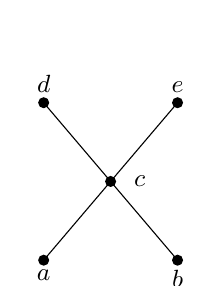
\begin{tikzpicture}[scale=1.0,every node/.style={font=\small}]
\coordinate (a) at (-0.85,0);\coordinate (b) at (0.85,0);
\coordinate (c) at (0,1);\coordinate (d) at (-0.85,2);\coordinate (e) at (0.85,2);
\draw (a)--(c)--(d) (b)--(c)--(e);
\foreach \v in {a,b,c,d,e}{\fill (\v) circle(2pt);}
\node[below] at (a) {$a$};\node[below] at (b) {$b$};
\node[right=5pt] at (c) {$c$};\node[above] at (d) {$d$};\node[above] at (e) {$e$};
\end{tikzpicture}
\caption{The five-element extremizer $X$. Here $h(X)=\sO(X)=3$ but $\sC(X)=4$.}\label{fig:X}
\end{figure}

The chain-polytope facet
\[
x_b+x_c+x_e=1
\]
has precisely the five vertices
\[
e_b,\quad e_a+e_b,\quad e_c,\quad e_e,\quad e_d+e_e.
\]
They are affinely independent, so this is a $4$-simplex. In the order polytope, the equations $x_b=x_c=x_d$ define a $3$-simplex with vertices
\[
\zero,\quad e_e,\quad e_b+e_c+e_d+e_e,\quad\one.
\]
The state recursion gives $M(X)=\smat{3}{3}{3}{3}$ and excludes all larger simplex faces. These explicit witnesses help distinguish the positive result from a purely numerical optimization report.

\section{Algorithms, certificates, and reproducibility}\label{sec:algorithms}

\subsection{Evaluation from a supplied decomposition}
A binary decomposition tree has $n$ singleton leaves and $n-1$ operation nodes. At each node store
\[
\bigl(n(P),M(P),h(P),u(P)\bigr).
\]
Use \cref{thm:chain,thm:orderseries,thm:orderparallel}. Each node needs a bounded number of additions and comparisons. All finite values lie between $-1$ and $n$. Thus evaluation takes $O(n)$ arithmetic operations, or $O(n\log n)$ bit operations with an elementary integer-cost accounting. A postorder implementation uses $O(n)$ stored machine words, or less when values are discarded after use.

This bound is for a supplied decomposition, not for discovering the decomposition from an arbitrary representation of a poset. It is also not a claim that explicitly listing all coordinates of a large witness takes linear bit time.

The reference implementation uses immutable expression trees, for example:
\par\noindent\begin{minipage}{\linewidth}
\begin{lstlisting}[language=Python]
from simplex_posets import evaluate, layered_expr, layered_formula

P = layered_expr([2, 1, 2])
answer = evaluate(P)
assert answer.order_simplex == 3
assert answer.chain_simplex == 4
assert answer.matrix == (3, 3, 3, 3)

# Entries are (m00, m01, m10, m11), in row-major order.
assert layered_formula([2, 3, 2, 1, 2, 2, 3]) == (10, 12, 3)
\end{lstlisting}
\end{minipage}\par

The library also accepts expressions \texttt{'x'}, \texttt{('S', A, B)}, and \texttt{('P', A, B)}, denoting a singleton, ordinal sum, and disjoint union, respectively. The direct numerical result can be obtained without enumerating filters, antichains, or faces.

\subsection{Recovering a decomposition}
The supplied implementation includes a simple recognition procedure. Split a poset into connected components of its comparability graph when possible; this is a disjoint union. Otherwise split its incomparability graph into components when possible; these components are totally ordered and give an ordinal sum. Recurse. If neither graph splits and the poset has more than one element, it is not series--parallel under our definition.

For completeness, the ordering assertion follows from transitivity. If $x$ and $y$ are incomparable and $z$ is in a different incomparability component, $z$ is comparable with both. It cannot lie strictly between them, because that would force $x$ and $y$ to be comparable. Hence its comparison direction is the same along an incomparability edge, and therefore along an entire component. Applying this in both components shows that every cross-comparison has one common direction. The component order is consequently linear.

Any series--parallel expression with more than one leaf has a root operation that disconnects one of the two graphs. Therefore the recursive recognition is complete. Conversely, every successful split constructs a valid expression. The deliberately elementary implementation has a conservative $O(n^3)$ bound using a full transitive-relation representation; the article does not claim a sharper recognition bound for this code.

\subsection{Constructive witness recovery}
Every maximum in the recurrences is attained by finitely many candidate faces. Recording a maximizing alternative at each node therefore recovers an optimal simplex inductively. Product steps fix a vertex in the inactive factor. An ordinal-sum step combines the two chosen component simplices, identifying their common vertex in the through-vertex case, or taking their join in the avoiding case.

The theorem is constructive even without a general witness routine in the fast evaluator. The distributed geometry checker does output explicit maximizing vertex sets and active defining inequalities for selected examples. It verifies those certificates independently of the recurrence.

\subsection{Independent exact geometric verification}\label{sec:independent}
The main verification does \emph{not} merely compare one implementation of a recurrence with another. For each test poset it builds the complete vertex lists from \cref{lem:vertices} and the defining inequalities of \eqref{eq:orderdef} or \eqref{eq:chaindef}. All strict order comparisons may be used in the former, and all maximal chains in the latter. Redundant valid inequalities cause no problem.

For any nonempty set $W$ of vertices, intersect all defining inequalities that are tight at every vertex of $W$. The resulting face is the smallest face containing $W$. The checker represents it by the complete set of vertices satisfying these common equalities. In particular, a pair of vertices is an edge exactly when this smallest face has precisely those two vertices.

It then solves an exact maximum-clique problem in this geometrically recovered edge graph, separately for every prescribed endpoint state. A simplex face necessarily gives a clique, so this supplies an upper bound. For each optimizing clique, the checker additionally verifies that its smallest containing face has no extra vertices and that its affine rank is the clique size minus one. Thus the optimizing clique is itself a simplex face, proving attainment of the upper bound.

Although Mori's clique characterization~\cite{Mori2025} would justify skipping the last step, we deliberately retain the geometric certification. No specialized clique-face theorem or series--parallel recurrence is used to compute the geometric answers. Ranks are computed over rational numbers, not with a floating-point tolerance. The only floating-point sentinel in the library is $-\infty$ for an impossible state.

\subsection{Exhaustive coverage and actual results}
A poset is naturally labelled if $i<_Pj$ implies $i<j$ as integers. All naturally labelled posets are generated recursively: add a new greatest-labelled element and choose its strict lower set to be any order ideal of the old poset. This generates every naturally labelled transitive relation exactly once. Every finite poset admits such a labelling, so this covers every isomorphism type, possibly repeatedly.

The full verification run generated all such posets through six elements, retained those recognized as series--parallel, and compared all four order states and both chain states. The results were:

\begin{table}[htbp]
\centering
\caption{Exact verification from defining inequalities. Certificates count feasible endpoint states, including the empty simplex when optimal.}\label{tab:geometry}
\begin{tabular}{rrrrr}
\toprule
$n$ & All natural posets & SP instances & Pair-face tests & Face certificates\\
\midrule
1 & 1 & 1 & 2 & 6\\
2 & 2 & 2 & 18 & 11\\
3 & 7 & 7 & 198 & 38\\
4 & 40 & 35 & 2,740 & 188\\
5 & 357 & 223 & 45,566 & 1,187\\
6 & 4,824 & 1,709 & 885,238 & 9,026\\
\midrule
Total & 5,231 & 1,977 & 933,762 & 10,456\\
\bottomrule
\end{tabular}
\end{table}

All comparisons passed. Thirty additional seeded series--parallel examples, ten each on seven, eight, and nine elements, also passed, with 562,028 further pair-face tests. The seed is recorded as \texttt{20260920}; the samples are not asserted to be uniformly distributed over posets.

A separate signature saturation uses only the recurrences: for each size, it combines every signature from all smaller size splits and merges duplicates. It is complete for the attainable signatures, not a count of nonisomorphic posets. Through size fifteen, it found the values in \cref{tab:signatures}. Every signature satisfied the eight-state restriction, the exceptional-case invariant, the potential inequality, and the sharp gap bound.

\begin{table}[htbp]
\centering
\caption{Complete signature saturation under the two operations.}\label{tab:signatures}
\begin{tabular}{rrr@{\qquad}rrr}
\toprule
$n$ & Signatures & Maximum gap & $n$ & Signatures & Maximum gap\\
\midrule
1 & 1 & 0 & 9 & 129 & 2\\
2 & 2 & 0 & 10 & 179 & 2\\
3 & 5 & 0 & 11 & 243 & 3\\
4 & 10 & 0 & 12 & 320 & 3\\
5 & 20 & 1 & 13 & 414 & 3\\
6 & 35 & 1 & 14 & 521 & 4\\
7 & 58 & 1 & 15 & 649 & 4\\
8 & 87 & 2 &  & & \\
\bottomrule
\end{tabular}
\end{table}

The closed layer formula was independently compared with the matrix recurrence for every word over $\{1,2,3\}$ of length at most nine: $3+3^2+\cdots+3^9=29,523$ words. The 64 series transitions and all 64 potential inequalities were checked exactly. As a check on the optimization infrastructure, 250 seeded small-graph clique problems with endpoint constraints were compared with exhaustive subset enumeration. The iterative evaluator also passed a 5,000-element chain test. Explicit extremizers were also checked for each $2\le n\le100$. These are regression checks of the formulae and implementations; the proofs, rather than the finite range of testing, establish the unbounded statements.

\subsection{Running the archive}
The code requires Python 3.10 or newer and only its standard library. From the archive directory run:
\begin{lstlisting}
python verify.py --full --output reproduced_results
\end{lstlisting}
A smaller smoke test is available as \texttt{python verify.py --quick}. The full run that produced the included files reported Python 3.13.5 and an elapsed time of approximately 4.1 seconds in the execution environment used for this draft. That timing is an observation, not a portable performance guarantee.

The directory \texttt{results/} contains a structured report, the transition certificate, and explicit geometric witnesses. The file \texttt{verification.log} records the completed run. A Makefile supplies targets for compilation and verification. No proprietary solver, external service, or network access is needed to reproduce the computations.

\section{What is established, and what remains open}\label{sec:limits}

The stated series--parallel formula question has a concrete answer in two complementary forms. For all series--parallel posets there is a constant-state recursion, with a proof of its geometric meaning and a linear arithmetic-operation evaluation bound on a supplied decomposition. For ordinal sums of antichains, a path formula removes the recursion entirely. The sharp extremal theorem then identifies the exact largest discrepancy at each size across the full series--parallel class.

The geometric recurrences themselves hold for ordinal sums and disjoint unions of \emph{arbitrary} nonempty finite factors. Thus they also evaluate any decomposition whose leaf posets have already had their endpoint data computed. What is special about singleton-generated series--parallel posets is the eight-state closure and the resulting uniform potential inequality. We have not established that closure, the same sharp gap bound, or an efficient base-case computation for arbitrary indecomposable finite posets.

Several distinctions prevent overinterpretation. The dimension inequality is weaker than the existing dimension-by-dimension simplex-count inequality, and our proof does not settle the unrestricted Hibi--Li face-number conjecture. Equality of $\sO$ and $\sC$ does not imply affine equivalence. The running-time theorem does not treat a compressed exponentially large decomposition as an ordinary $n$-node input. And none of the constructions automatically extends to infinite ordinal sums, where compactness, the definition of a polyhedral face, and finiteness of vertex sets would all require reconsideration.

The most immediate further mathematical question is whether the extremal gap bound survives outside the series--parallel class. The present proof neither establishes nor refutes that extension. Another question is to characterize all extremizers, rather than give one attaining family at each size. The explicit states provide a practical starting point for both questions without treating computational evidence as a substitute for proof.

\appendix
\section{The complete finite potential certificate}\label{app:certificate}
For a transition $(a,b)\mapsto(c,\delta)$ define its slack by
\[
\sigma(a,b)=\kappa_a+\kappa_b-3+3\delta-\kappa_c.
\]
The following table lists every slack. Since all are nonnegative, it proves all instances of \eqref{eq:finitepotential}. Together with the symbolic recurrence and the displayed state matrices, it is a small certificate that can be checked without running the code.

\begin{table}[htbp]
\centering
\caption{Nonnegative slacks $\sigma(a,b)$ for the potential induction.}\label{tab:slacks}
\renewcommand{\arraystretch}{1.2}
\begin{tabular}{c|rrrrrrrr}
\toprule
$a\backslash b$ &1&2&3&4&5&6&7&8\\
\midrule
1 & 1 & 1 & 0 & 1 & 0 & 1 & 1 & 0\\
2 & 1 & 1 & 1 & 1 & 0 & 1 & 2 & 1\\
3 & 1 & 1 & 0 & 1 & 0 & 1 & 1 & 0\\
4 & 0 & 1 & 2 & 0 & 1 & 2 & 3 & 2\\
5 & 0 & 0 & 1 & 0 & 0 & 1 & 2 & 1\\
6 & 1 & 1 & 2 & 1 & 1 & 2 & 3 & 2\\
7 & 1 & 2 & 3 & 1 & 2 & 3 & 4 & 3\\
8 & 0 & 1 & 2 & 0 & 1 & 2 & 3 & 2\\
\bottomrule
\end{tabular}
\end{table}

The constants are not presented as an optimized or unique choice of potential. Their role is to give a readily verifiable induction with minimum constant two. That minimum, combined with the exact coefficient three in the potential, is precisely what produces the global upper bound $(n-2)/3$.

\section{Archive contents and conventions}\label{app:archive}
The main article source is \texttt{Largest\_Simplex\_Faces.tex}, compiled to the correspondingly named PDF. The source is self-contained apart from standard LaTeX packages; the bibliography and all numerical tables are embedded. The file \texttt{simplex\_posets.py} contains the formula evaluator, finite-poset operations, exact face checker, and rational rank computation. The file \texttt{verify.py} runs the regression suite.

The JSON file \texttt{results/transitions.json} records the 64 state transitions, increments, and potential slacks. The file \texttt{results/verification.json} records test ranges, counts, and the successful completion status. The file \texttt{results/examples.json} records the geometric witnesses for six selected layered examples, including $X$ and the orientation-sensitive pair from \cref{sec:counterexample}.

Elements in the machine-readable certificates are numbered starting at zero. An inequality is stored as an integer coefficient vector $a$ and a right-hand side $b$, meaning $a\cdot x\le b$. Vertices are stored as lists of coordinates equal to one. An impossible state is serialized as the string \texttt{"-infinity"}; the empty simplex is separately marked and has dimension $-1$. These conventions avoid conflating infeasibility with the empty face.

\begin{thebibliography}{99}
\bibitem{Stanley1986}
R.~P. Stanley, \emph{Two poset polytopes}, Discrete \& Computational Geometry \textbf{1} (1986), 9--23.
\href{https://doi.org/10.1007/BF02187680}{doi:10.1007/BF02187680}.

\bibitem{FHL2026}
R.~Freij-Hollanti and T.~Lundstr\"om, \emph{Simplex inequalities of order and chain polytopes of recursively defined posets}, Order \textbf{43} (2026), article 31. Published 2 September 2026. The open question used here is in Section~4, printed page 9 of 10.
\href{https://doi.org/10.1007/s11083-026-09744-1}{doi:10.1007/s11083-026-09744-1}.

\bibitem{FHLpreprint}
R.~Freij-Hollanti and T.~Lundstr\"om, \emph{Simplex inequalities of order and chain polytopes of recursively defined posets}, arXiv:2511.03557, version~1, 5 November 2025.
\href{https://arxiv.org/abs/2511.03557}{arXiv:2511.03557}.

\bibitem{FHL2024}
R.~Freij-Hollanti and T.~Lundstr\"om, \emph{$f$-vector inequalities for order and chain polytopes}, Mathematica Scandinavica \textbf{130} (2024), no.~3, 467--486.
\href{https://doi.org/10.7146/math.scand.a-143995}{doi:10.7146/math.scand.a-143995}.

\bibitem{Mori2025}
A.~Mori, \emph{Simplex faces of order and chain polytopes}, Order \textbf{42} (2025), 805--810.
\href{https://doi.org/10.1007/s11083-025-09709-w}{doi:10.1007/s11083-025-09709-w}.
Preprint: \href{https://arxiv.org/abs/2307.08447}{arXiv:2307.08447}.

\bibitem{MoriOhsugi2026}
A.~Mori and H.~Ohsugi, \emph{Simplex faces and quadratic toric ideals of lattice polytopes}, arXiv:2606.20430, version~3, 22 July 2026.
\href{https://arxiv.org/abs/2606.20430}{arXiv:2606.20430}.

\bibitem{Jung1978}
H.~A. Jung, \emph{On a class of posets and the corresponding comparability graphs}, Journal of Combinatorial Theory, Series~B \textbf{24} (1978), no.~2, 125--133.
\href{https://doi.org/10.1016/0095-8956(78)90013-8}{doi:10.1016/0095-8956(78)90013-8}.
\end{thebibliography}
\end{document}
